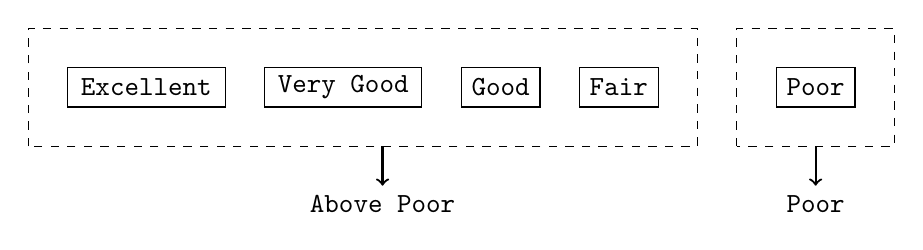
\begin{tikzpicture}
    % Define the font style
    \tikzstyle{every node}=[font=\ttfamily]
  
    % Draw the rectangles for each answer option
    \draw (0,0) rectangle (2,0.5) node[midway] {Excellent};
    \draw (2.5,0) rectangle (4.5,0.5) node[midway] {Very Good};
    \draw (5,0) rectangle (6,0.5) node[midway] {Good};
    \draw (6.5,0) rectangle (7.5,0.5) node[midway] {Fair};
    \draw (9,0) rectangle (10,0.5) node[midway] {Poor};
  
    \pause
    % Draw the dashed rectangles around the grouped answer options
    \draw[dashed] (-0.5,-0.5) rectangle (8,1);
    \draw[dashed] (8.5,-0.5) rectangle (10.5,1);
  
    % Add arrows pointing downwards from the middle of the dashed rectangles
    \draw[->, thick] (4,-0.5) -- (4,-1) node[below] {Above Poor};
    \draw[->, thick] (9.5,-0.5) -- (9.5,-1) node[below] {Poor};
\end{tikzpicture}